\documentclass[a4paper, 12pt, twoside]{article}
\usepackage[T2A,T1]{fontenc}
\usepackage[utf8]{inputenc}
\usepackage[english, russian]{babel}
\usepackage{graphicx}
\usepackage[hcentering, bindingoffset = 10mm, right = 15 mm, left = 15 mm, top=20mm, bottom = 20 mm]{geometry}
\usepackage{multirow}
\usepackage{lipsum}
\usepackage{amsmath, amstext}
\usepackage{siunitx}
\usepackage{subcaption}
\usepackage{wrapfig}
\usepackage{adjustbox}
\usepackage{enumerate, indentfirst, float}
\usepackage{capt-of, svg}
\usepackage{cmap} % Улучшенный поиск русских слов в полученном pdf-файле

\usepackage{pscyr} % Нормальные шрифты
\usepackage[normalem]{ulem} % для подчёркиваний uline
\ULdepth = 0.16em

\usepackage{fancyhdr} %Колонтикулы
\pagestyle{fancy}
\lhead{
\includegraphics[width = 10 mm]{logo.jpg} Лабораторная работа № 3.2.4}
\rhead{\textit{\today}}

\newenvironment{bottompar}{\par\vspace*{\fill}}{\clearpage}
 
\begin{document}
\begin{titlepage}

\newcommand{\HRule}{\rule{\linewidth}{0.7mm}} % Defines a new command for the horizontal lines, change thickness here

\center % Center everything on the page
 
%----------------------------------------------------------------------------------------
%	HEADING SECTIONS
%----------------------------------------------------------------------------------------

\textsc{\LARGE Московский Физико-Технический Институт}\\[1,5cm] % Name of your university/college
\textsc{\Large Кафедра общей физики}\\[0.5cm] % Major heading such as course name
\textsc{\large Лабораторная работа \textnumero  3.2.4}\\[0.5cm] % Minor heading such as course title

%----------------------------------------------------------------------------------------
%	TITLE SECTION
%----------------------------------------------------------------------------------------

\HRule
\\[0.4cm]
{ \huge \bfseries Свободные колебания в электрическом контуре.}
\\[0.2cm] % Title of your document
\HRule
\\[1.5cm]


 
%----------------------------------------------------------------------------------------
%	AUTHOR SECTION
%----------------------------------------------------------------------------------------

\begin{minipage}{0.4\textwidth}
	\begin{flushleft} \large
		\textbf{Автор:}\\
		Глеб Уваркин \\
		615 группа
	\end{flushleft}
\end{minipage}
~
\begin{minipage}{0.4\textwidth}
	\begin{flushright} \large
		\textbf {Преподаватель:} \\
		Андрей Александрович Заболотных % Supervisor's Name
	\end{flushright}
\end{minipage}

\begin{bottompar}
	\begin{center}
		
\includegraphics[width = 80 mm]{logo.jpg}
	\end{center}
	{\large \today}

\end{bottompar}
\vfill % Fill the rest of the page with whitespace

\end{titlepage}

{\Large \uline { \textbf  {Цель работы:}}}

\vspace{2mm}

Исследование свободных колебаний в колебательном контуре.

\vspace{\baselineskip}

{\Large \uline { \textbf  {В работе используются:}}}

\vspace{2mm}

Генератор импульсов, электронное реле, магазин сопротивлений, магазин ёмкостей, индуктивность, электронный осциллограф с разделительной панелью, измеритель {\textit{LCR}}.

\section{Теоретические сведения.}
\subsection{Предмет исследования.}
\begin{wrapfigure}{r}{0.2\linewidth}
	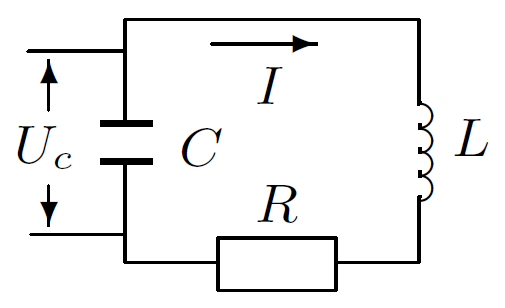
\includegraphics[width = \linewidth]{RLC}
	\caption{Колебательный контур.}
	\label{RLC}
\end{wrapfigure}
В этой лабораторной работе мы будем рассматривать гармонические колебания токов(зарядов) в электрических цепях, включающих в себя резисторы , конденсаторы и катушки индуктивности(рис. \ref{RLC}). Все колебания мы будем рассматривать при относительно низких частотах когда выполняется условие {\textit{квазистационарности}}. Квазистационарность означает, что мгновенные значения тока $I$ практически одинаковы во всех проводниках, соединяющих элементы цепи, а изменения во времени происходя настолько медленно, что распространение электродинамических взаимодействий можно считать \textit{мгновенным}.

\begin{figure}[H]
	\centering
	\begin{minipage}[h]{0.3\linewidth}
		\centering{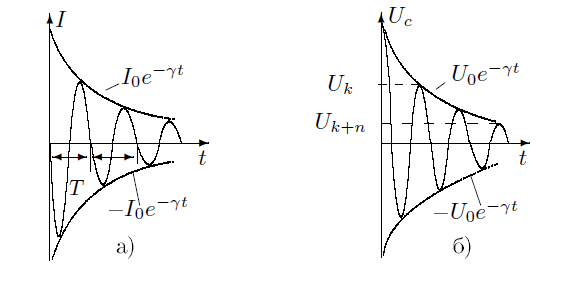
\includegraphics[width=0.9\linewidth]{kol.png} \\ а) Затухающие колебания($\gamma < \omega_{0}$)}
	\end{minipage}
	\begin{minipage}[h]{0.34\linewidth}
		\centering{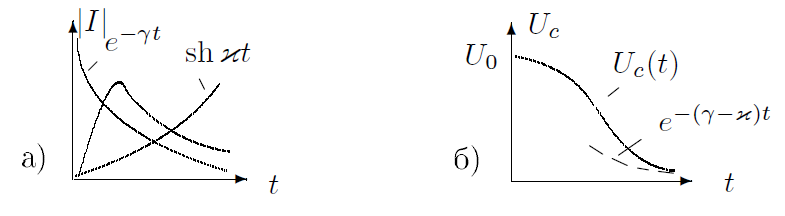
\includegraphics[width=0.9\linewidth]{aper.png} \\ б) Апериодический режим($\gamma > \omega_{0}$)}
	\end{minipage}
	\begin{minipage}[h]{0.34\linewidth}
		\centering{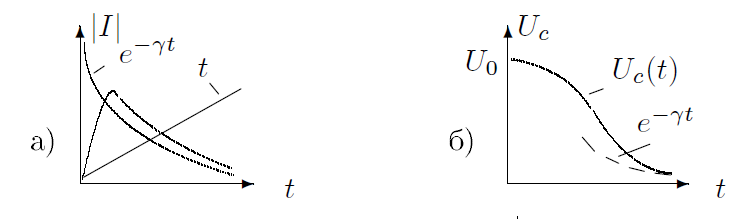
\includegraphics[width=0.9\linewidth]{krit.png} \\ б) Критический режим($\gamma = \omega_{0}$)}
	\end{minipage}
	
\end{figure}

\subsection{Основные формулы.}
$$\ddot I + 2\gamma \dot I + \omega_{0}^2 I = 0$$ - дифференциальное уравнение свободных колебаний, где $ \gamma =\dfrac{ R}{2L} $ - коэффициент затухания, $ \omega_{0}^2=
\dfrac{1}/{LC} $-собственная частота контура.

$$\omega = \sqrt{\omega_{0}^2-\gamma^2}$$ - частота свободных или собственных колебаний.

$$ R_{\text{кр}} = 2\sqrt{\dfrac{L}{C}}$$ - критическое сопротивление(сопротивление, при котором $\gamma = \omega_{0}$, а периодические колебания сменяются апериодическими).

В колебательном режиме потери в контуре принято характеризовать \textit{добротностью} и \textit{логарифмическим декрементом затухания}. Определим эти понятия. Назовём добротностью величину $$Q = 2\pi \dfrac{W}{\Delta W}$$

или

$$Q=\dfrac{1}{R}\sqrt {\dfrac{L}{C}}$$.

Добротность контура $Q$ показывает, \textit{во сколько раз запасённая в контуре энергия превосходит среднюю потерю энергии за время, в течение которого фаза колебаний изменяется на один радиан}.

Введём \textit{логарифмический декремент затухания $\Theta$} - логарифм отношения двух последовательных максимальных отклонений в одну сторону.

$$\Theta = \ln{\dfrac{U_k}{U_{k+1}}} = \ln{e^{\gamma T}}$$

На практике для определения $\Theta$ удобно использовать отношение максимальных отклонений, разделённых целым числом периодов n: $$Q=\dfrac{1}{n}\ln{\dfrac{U_k}{U_{k+n}}}$$

Связь между $\Theta$ и $Q$:
$$Q=\dfrac{\pi}{\gamma T} = \dfrac{\pi}{\Theta}$$


\section{Экспериментальная установка.}

\begin{figure}[H]
	\centering
	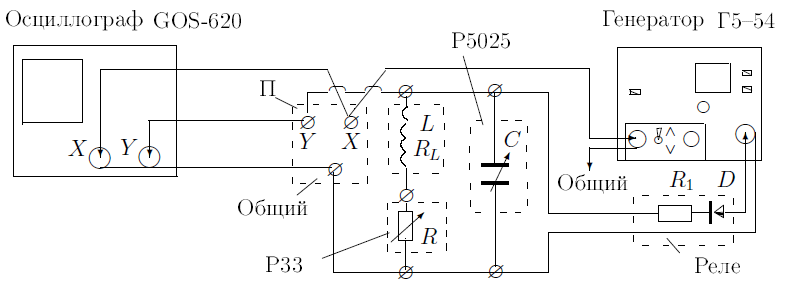
\includegraphics[width = 0.8\textwidth]{Schema}
	\caption{Схема установки для исследования свободных колебаний}
	\label{img:Schema}
\end{figure}

На рис.\ref{img:Schema} приведена схема дл исследования свободных колебаний в контуре, содержащем постоянную индуктивность $L$ и переменные ёмкость $C$ и сопротивление $R$. Колебания наблюдаются на экране осциллографа.

Для периодического возбуждения колебаний в контуре используется генератор импульсов Г5-54. С выхода генератора по коаксиальному кабелю и импульсы поступают на колебательный контур через электронное реле, смонтированное в отдельном блоке (или на выходе генератора). Реле содержит диодный тиристор $D$ и ограничительный резистор $R_{1}$.

Импульсы заряжают конденсатор $C$. После каждого импульса генератор отключается от колебательного контура и в контуре возникают свободные затухающие колебания. Входное сопротивление осциллографа велико ($\simeq 1$ МОм), так что его влиянием на контур можно пренебречь. Для получения устойчивой картины затухающих колебаний используется режим ждущей развертки с синхронизацией внешними импульсами, поступающими с выхода <<синхроимпульсы>> генератора.

\section{Ход работы.}

\subsection{Измерение периодов.}
Соберём схему согласно рис. \ref{img:Schema} , подготовим осциллограф к работе, установим длительность импульсов $\sim5\mu S$, частоту повторения импульсов $\nu_{0} = 100\text{Hz}$($T_{0} = 0,01\text{с}$).\\

Подберём частоту развертки ЭО, при которой расстояние $x_{0}$ между импульсами, поступающими с генератора, занимает почти весь экран($x_{0} = (10,4 \pm 0,2)\text{мс}$).

Изменяя ёмкость от 0,02 мкФ до 0,9 мкФ  и, периодически проверяя величину $x_{0}$, проведём измерение расстояния $x$, которое занимают несколько полных периодов $n$ и рассчитаем период колебаний контура по формуле:
\begin{equation} 
T=T_{0}x/(nx_{0})
\end{equation}

Полученные значения запишем в таблицу \ref{table1}.

\begin{table}[H]
	\centering
	\caption{Зависимость периода свободных колебаний контура от ёмкости конденсатора.}
	\label{table1}
	\begin{tabular}{|c|c|c|c|c|c|}
		\hline
		C, мкФ & x, мс & n  & T, мс & $\sigma_{T}$, мс & $\varepsilon$, \% \\ \hline
		0,02   & 4,7   & 14 & 0,32  & 0,01      & 3           \\ \hline
		0,11   & 8,6   & 11 & 0,75  & 0,02      & 2           \\ \hline
		0,20   & 9,4   & 9  & 1,00  & 0,02      & 2           \\ \hline
		0,29   & 8,8   & 7  & 1,21  & 0,03      & 2           \\ \hline
		0,38   & 8,6   & 6  & 1,38  & 0,04      & 2           \\ \hline
		0,47   & 8     & 5  & 1,54  & 0,04      & 2           \\ \hline
		0,56   & 8,8   & 5  & 1,69  & 0,04      & 2           \\ \hline
		0,65   & 7,6   & 4  & 1,83  & 0,04      & 2           \\ \hline
		0,74   & 8     & 4  & 1,92  & 0,04      & 2           \\ \hline
		0,83   & 8,6   & 4  & 2,07  & 0,05      & 2           \\ \hline
		0,9    & 9     & 4  & 2,16  & 0,05      & 2           \\ \hline
	\end{tabular}
\end{table}

\subsection{Критическое сопротивление и декремент затухания.}

Примем $L=200{\text{мГн}}$, найдём ёмкость $C$, при которой собственная частота колебаний контура $\nu_{0}$ составляет 5 кГц из формулы:
\begin{equation}
\nu_{0} = 1/(2\pi\sqrt{LC})
\end{equation}
$$ C = 0,005 \text{мкФ}$$

Для этих значений L и C рассчитаем критическое сопротивление контура $R_{кр}$ по формуле:
\begin{equation}
R_{\text{кр}} = 2\sqrt{L/C}
\end{equation}

$$ R_{\text{кр}} \approx 12,6 \text{кОм} $$

С помощью установки, собранной ранее, найдём экспериментальное значение сопротивления при котором колебательный режим переходит в апериодический:$$R_{\text{кр}} \approx 10 \text{кОм}$$ 

Для расчёта логарифмического декремента затухания $\Theta$ по формуле:
\begin{equation}
\label{form4}
\Theta = \frac{1}{n}\ln{\frac{U_{\text{k}}}{U_{\text{k+n}}}}
\end{equation}
измерим амплитуды, разделённые целым числом периодов $n$. Полученные значения запишем в таблицу \ref{table2}.

\begin{figure}[H]
	\centering
	\begin{minipage}[h]{0.49\linewidth}
		\centering{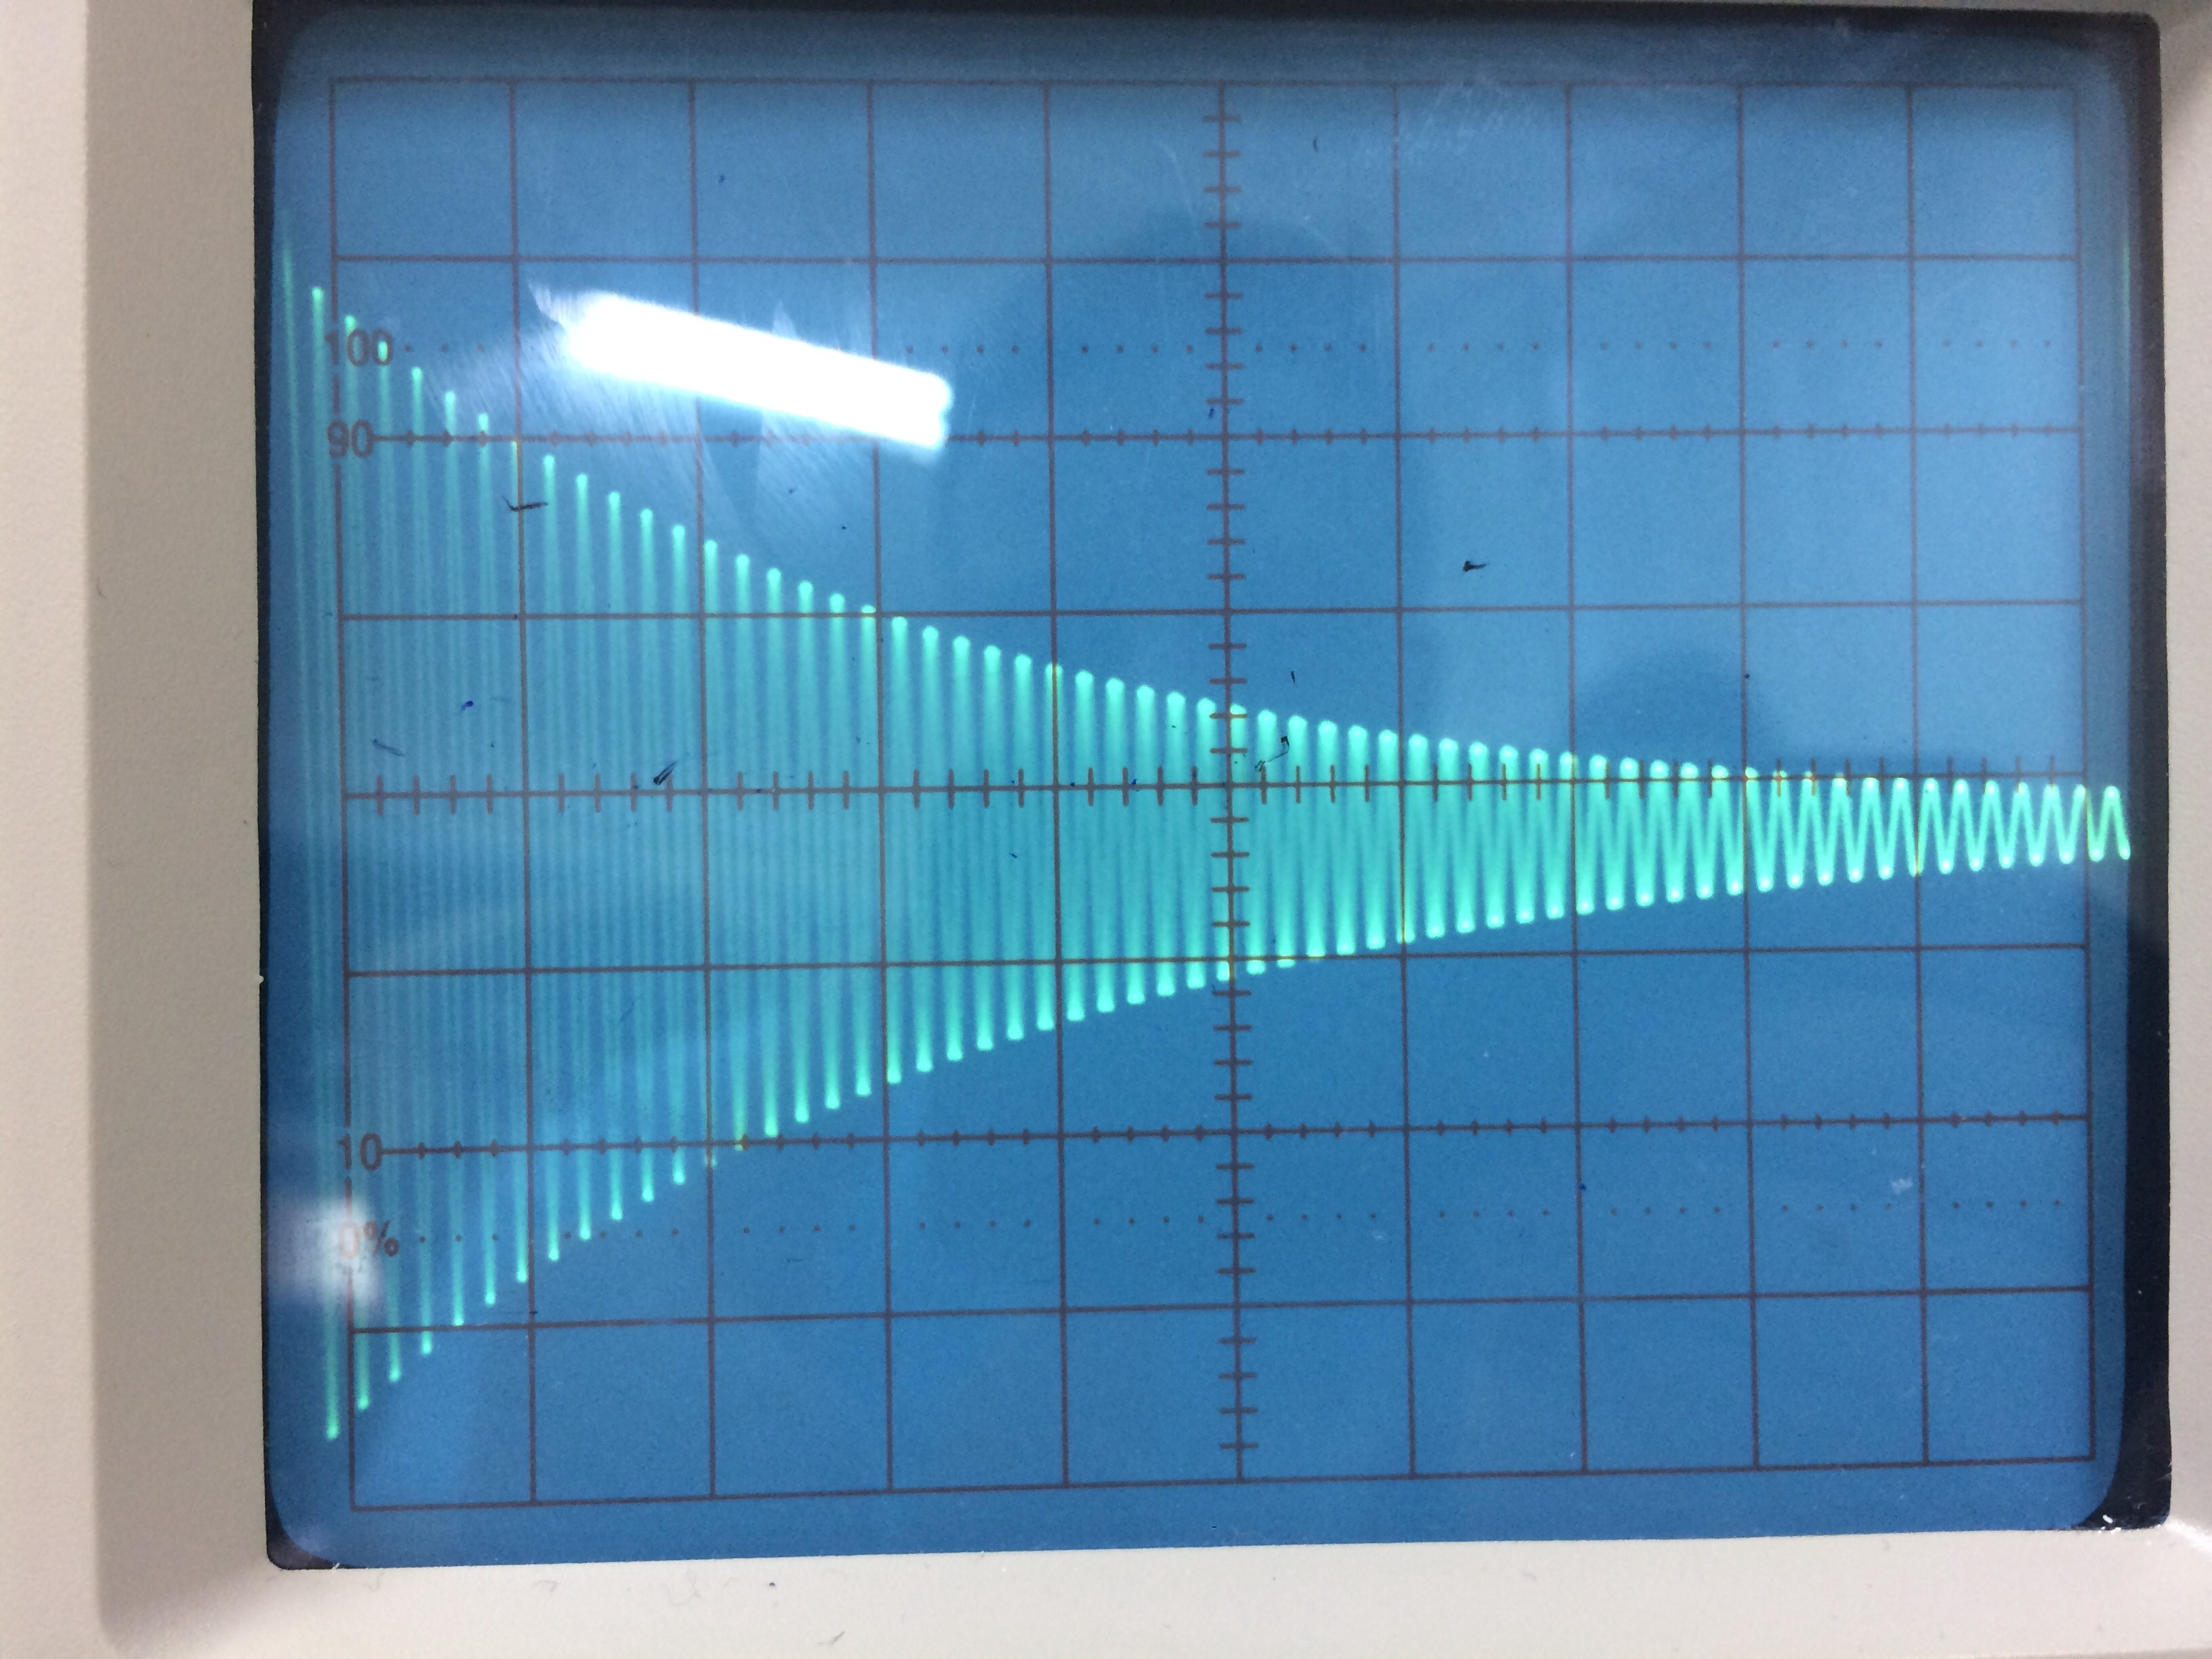
\includegraphics[width=0.9\linewidth]{IMG_0386} \\ а)$R = 0 ~ \text{Ом}$}
	\end{minipage}
	\begin{minipage}[h]{0.49\linewidth}
		\centering{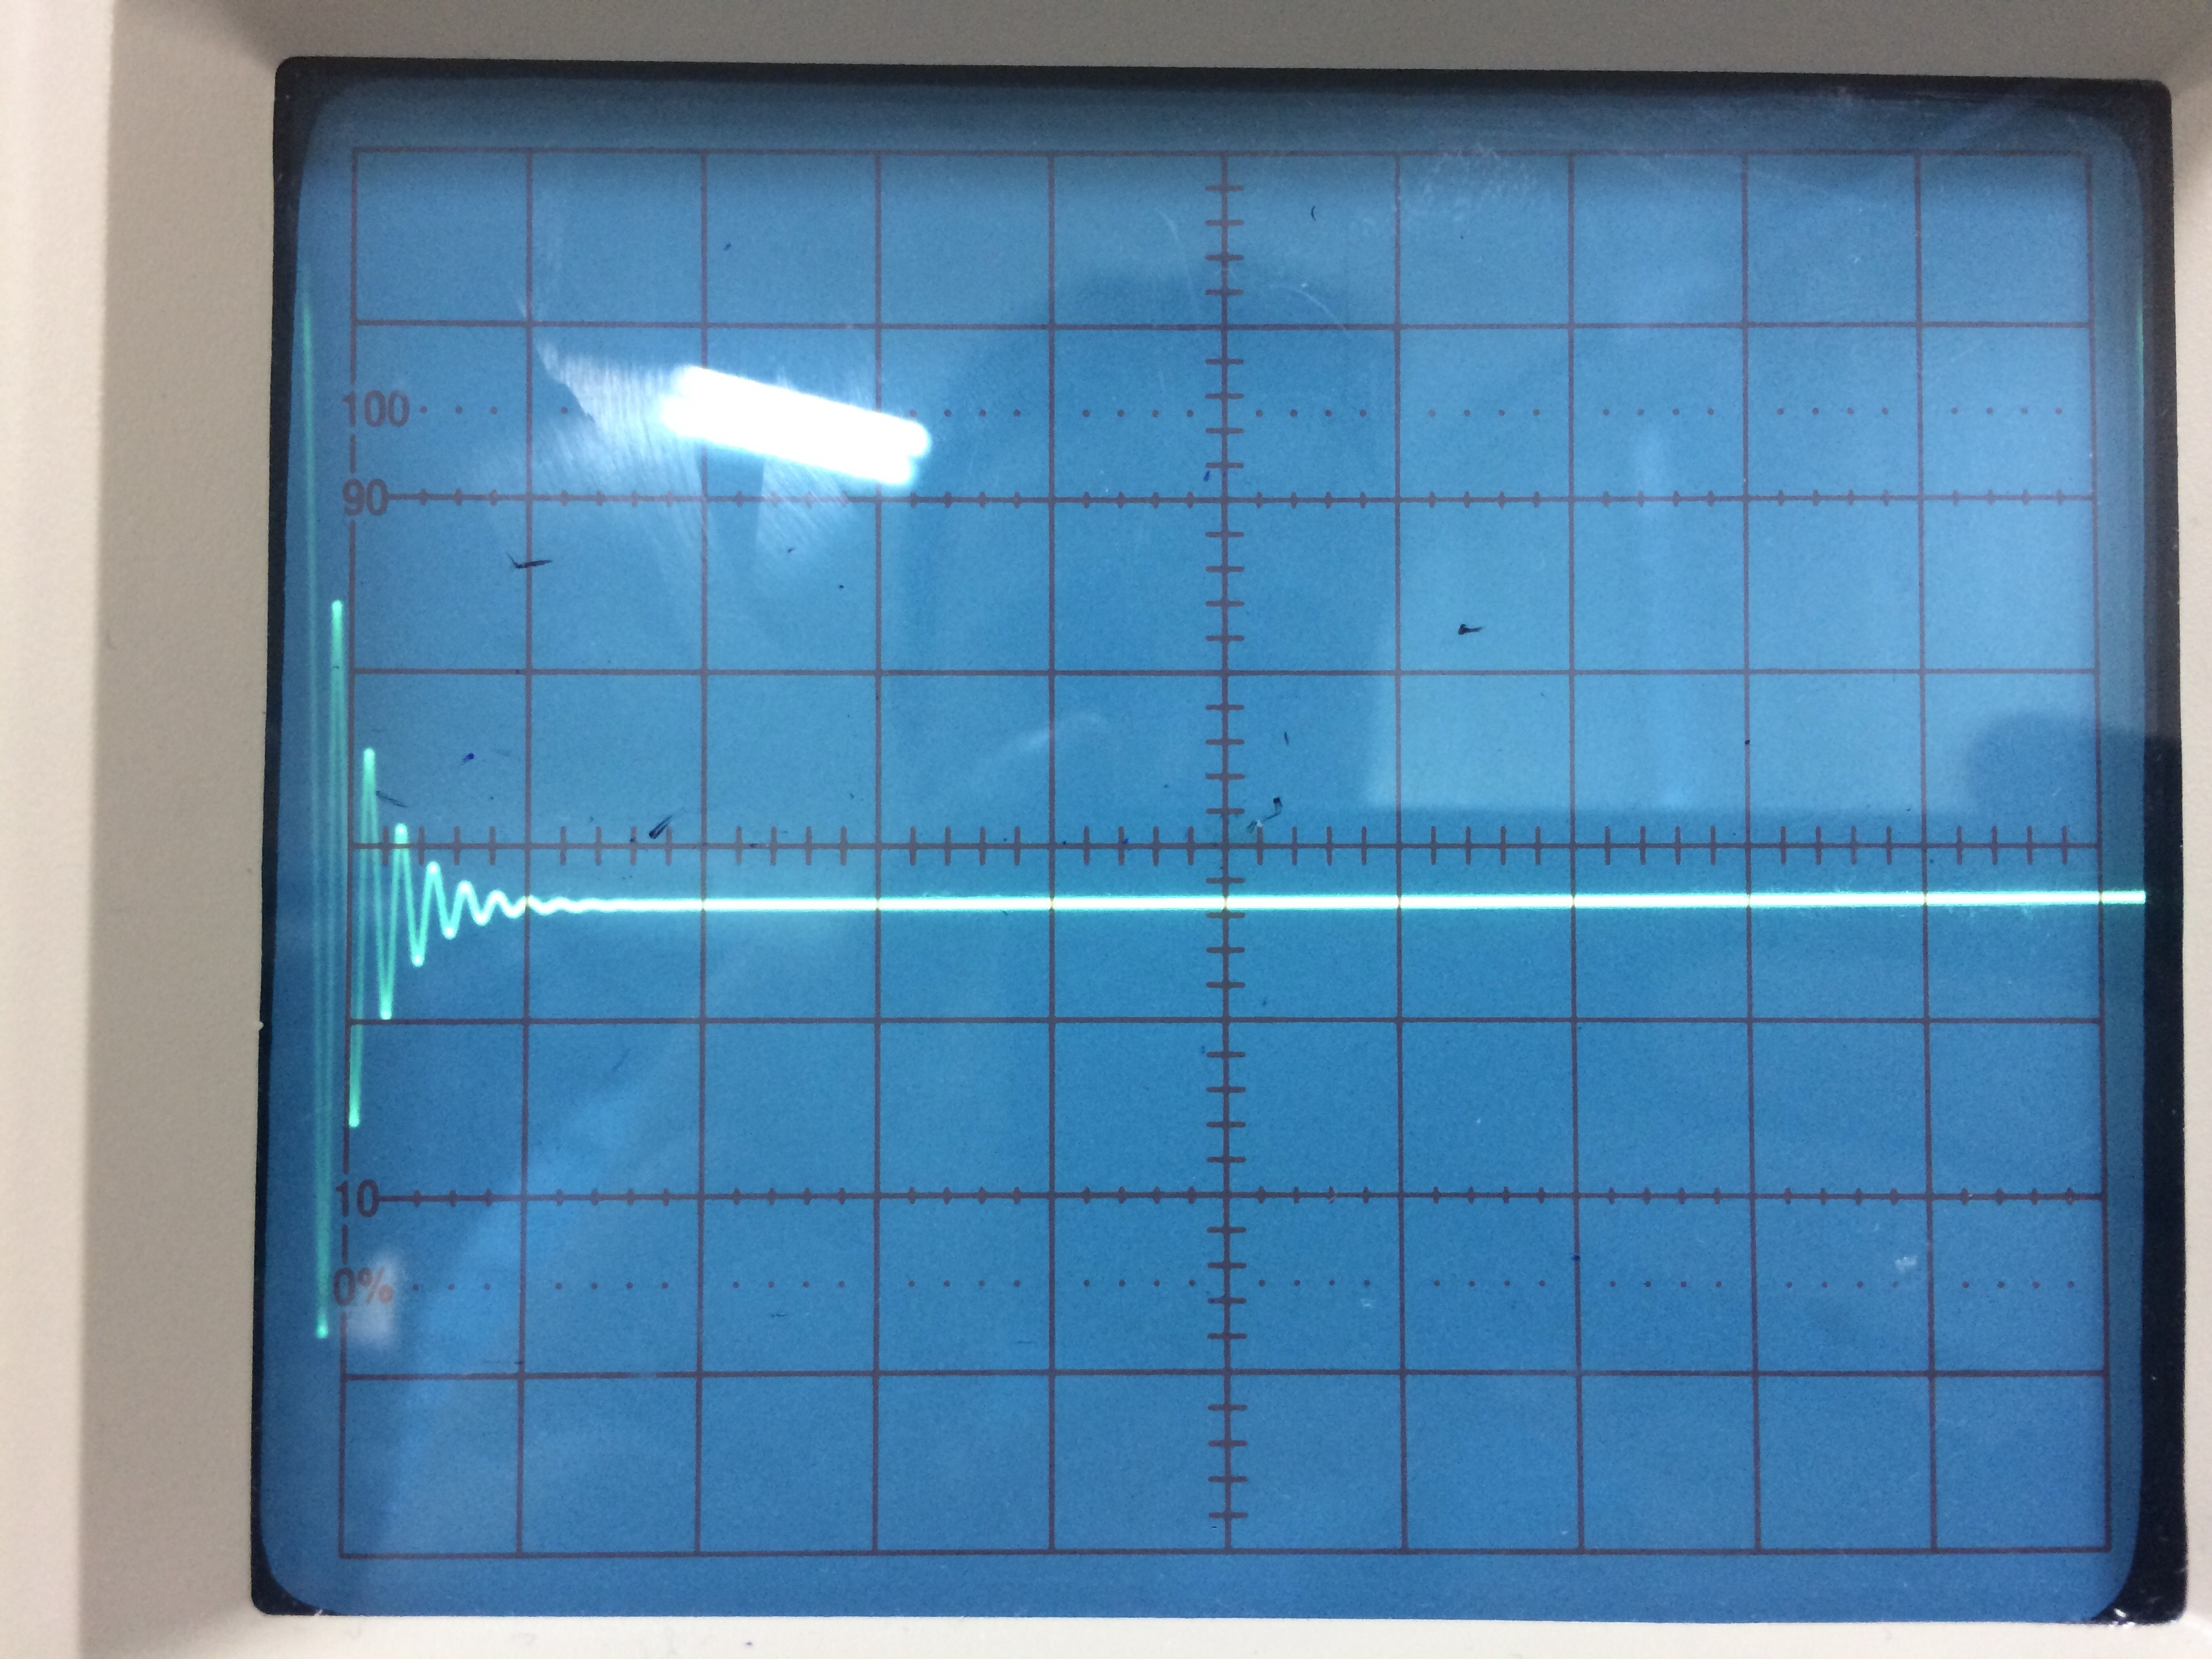
\includegraphics[width=0.9\linewidth]{IMG_0387} \\ б)$ R = 1000 ~ \text{Ом}$}
	\end{minipage}
	
	\caption{Вид свободных колебаний при разных значениях сопротивления $R$.}
	\label{ris:image1}
\end{figure}


\begin{table}[H]
	\centering
	\caption{Зависимость логарифмического декремента затухания $\Theta$ от сопротивления R.}
	\label{table2}
	\begin{tabular}{|c|c|c|c|c|}
		\hline
		R, кОм & $U_{0}$, дел & $U_{n}$, дел & n & $\Theta$   \\ \hline
		1      & 6,8     & 0,4     & 4 & 0,71    \\ \hline
		1,25   & 5,8     & 0,4     & 3 & 0,89    \\ \hline
		1,5    & 5       & 0,2     & 3 & 1,07    \\ \hline
		1,75   & 4,2     & 0,4     & 2 & 1,18    \\ \hline
		2      & 3,2     & 0,2     & 2 & 1,39    \\ \hline
		2,25   & 7,4     & 0,4     & 2 & 1,46    \\ \hline
		2,5    & 6,2     & 0,2     & 2 & 1,72    \\ \hline
		2,75   & 5,2     & 0,8     & 1 & 1,87   \\ \hline
		3      & 4,4     & 0,5     & 1 & 2,17    \\ \hline
	\end{tabular}
\end{table}

\subsection{Колебания на фазовой плоскости.}

Найдём логарифмический декремент затухания с помощью фазовой плоскости и формулы \ref{form4}. Для этого измерим радиусы витков спирали, разделённые целым числом периодов $n$. Данные запишем в таблицу \ref{table3}.

\begin{table}[H]
	\centering
	\caption{Измерение логарифмического декремента затухания $\Theta$ с помощью фазовой плоскости.}
	\label{table3}
	\begin{tabular}{|c|c|c|c|c|}
		\hline
		R, кОм & $r_{0}$, дел & $r_{n}$, дел & n &$\Theta$  \\ \hline
		1      & 4,6     & 1,2     & 2 & 0,67   \\ \hline
		1,25   & 5,6     & 1,1     & 2 & 0,81   \\ \hline
		2,75   & 4,2     & 0,6     & 1 & 1,95   \\ \hline
		3      & 4,6     & 0,6     & 1 & 2,04   \\ \hline
	\end{tabular}
\end{table}


Отсоединим катушку от цепи. Измерим омическое сопротивление катушки $R_{L}$ и индуктивность L с помощью измерителя \textit{LCR} на различных частотах.
\begin{table}[H]
	\centering
	\caption{Измерение характеристик катушки.}
	\label{table4}
	\begin{tabular}{|c|c|c|}
		\hline
		$\nu$, гц & L, мГн & R, Ом \\ \hline
		50    & 148,6  & 9,8   \\ \hline
		1000  & 142,73 & 12,2  \\ \hline
		5000  & 143,97 & 20,2  \\ \hline
	\end{tabular}
\end{table}

\section{Обработка результатов.}

\subsection{Исследование периода колебаний контура.}

Рассчитаем теоретические значения периода колебаний контура по формуле $$T=2\pi\sqrt{LC},$$ где $L\approx 145$мГн.

Сравним их с экспериментальными значениями, полученными в пункте \textbf{3.1}.

\begin{table}[H]
	\centering
	\caption{Сравнение теоретических и экспериментальных значений периода колебаний контура.}
	\label{table5}
	\begin{tabular}{|c|c|c|c|c|c|c|c|c|c|c|c|}
		\hline
		C, мкФ    & 0,02 & 0,11 & 0,20 & 0,29 & 0,38 & 0,47 & 0,56 & 0,65 & 0,74 & 0,83 & 0,90 \\ \hline
		$T_{\text{эксп}},$ мс & 0,32 & 0,75 & 1,00 & 1,21 & 1,38 & 1,54 & 1,69 & 1,83 & 1,92 & 2,07 & 2,16 \\ \hline
		$T_{\text{теор}},$ мс & 0,34 & 0,79 & 1,07 & 1,29 & 1,47 & 1,64 & 1,79 & 1,93 & 2,06 & 2,18 & 2,27 \\ \hline
	\end{tabular}
\end{table}

\begin{figure}[H]
	\centering
	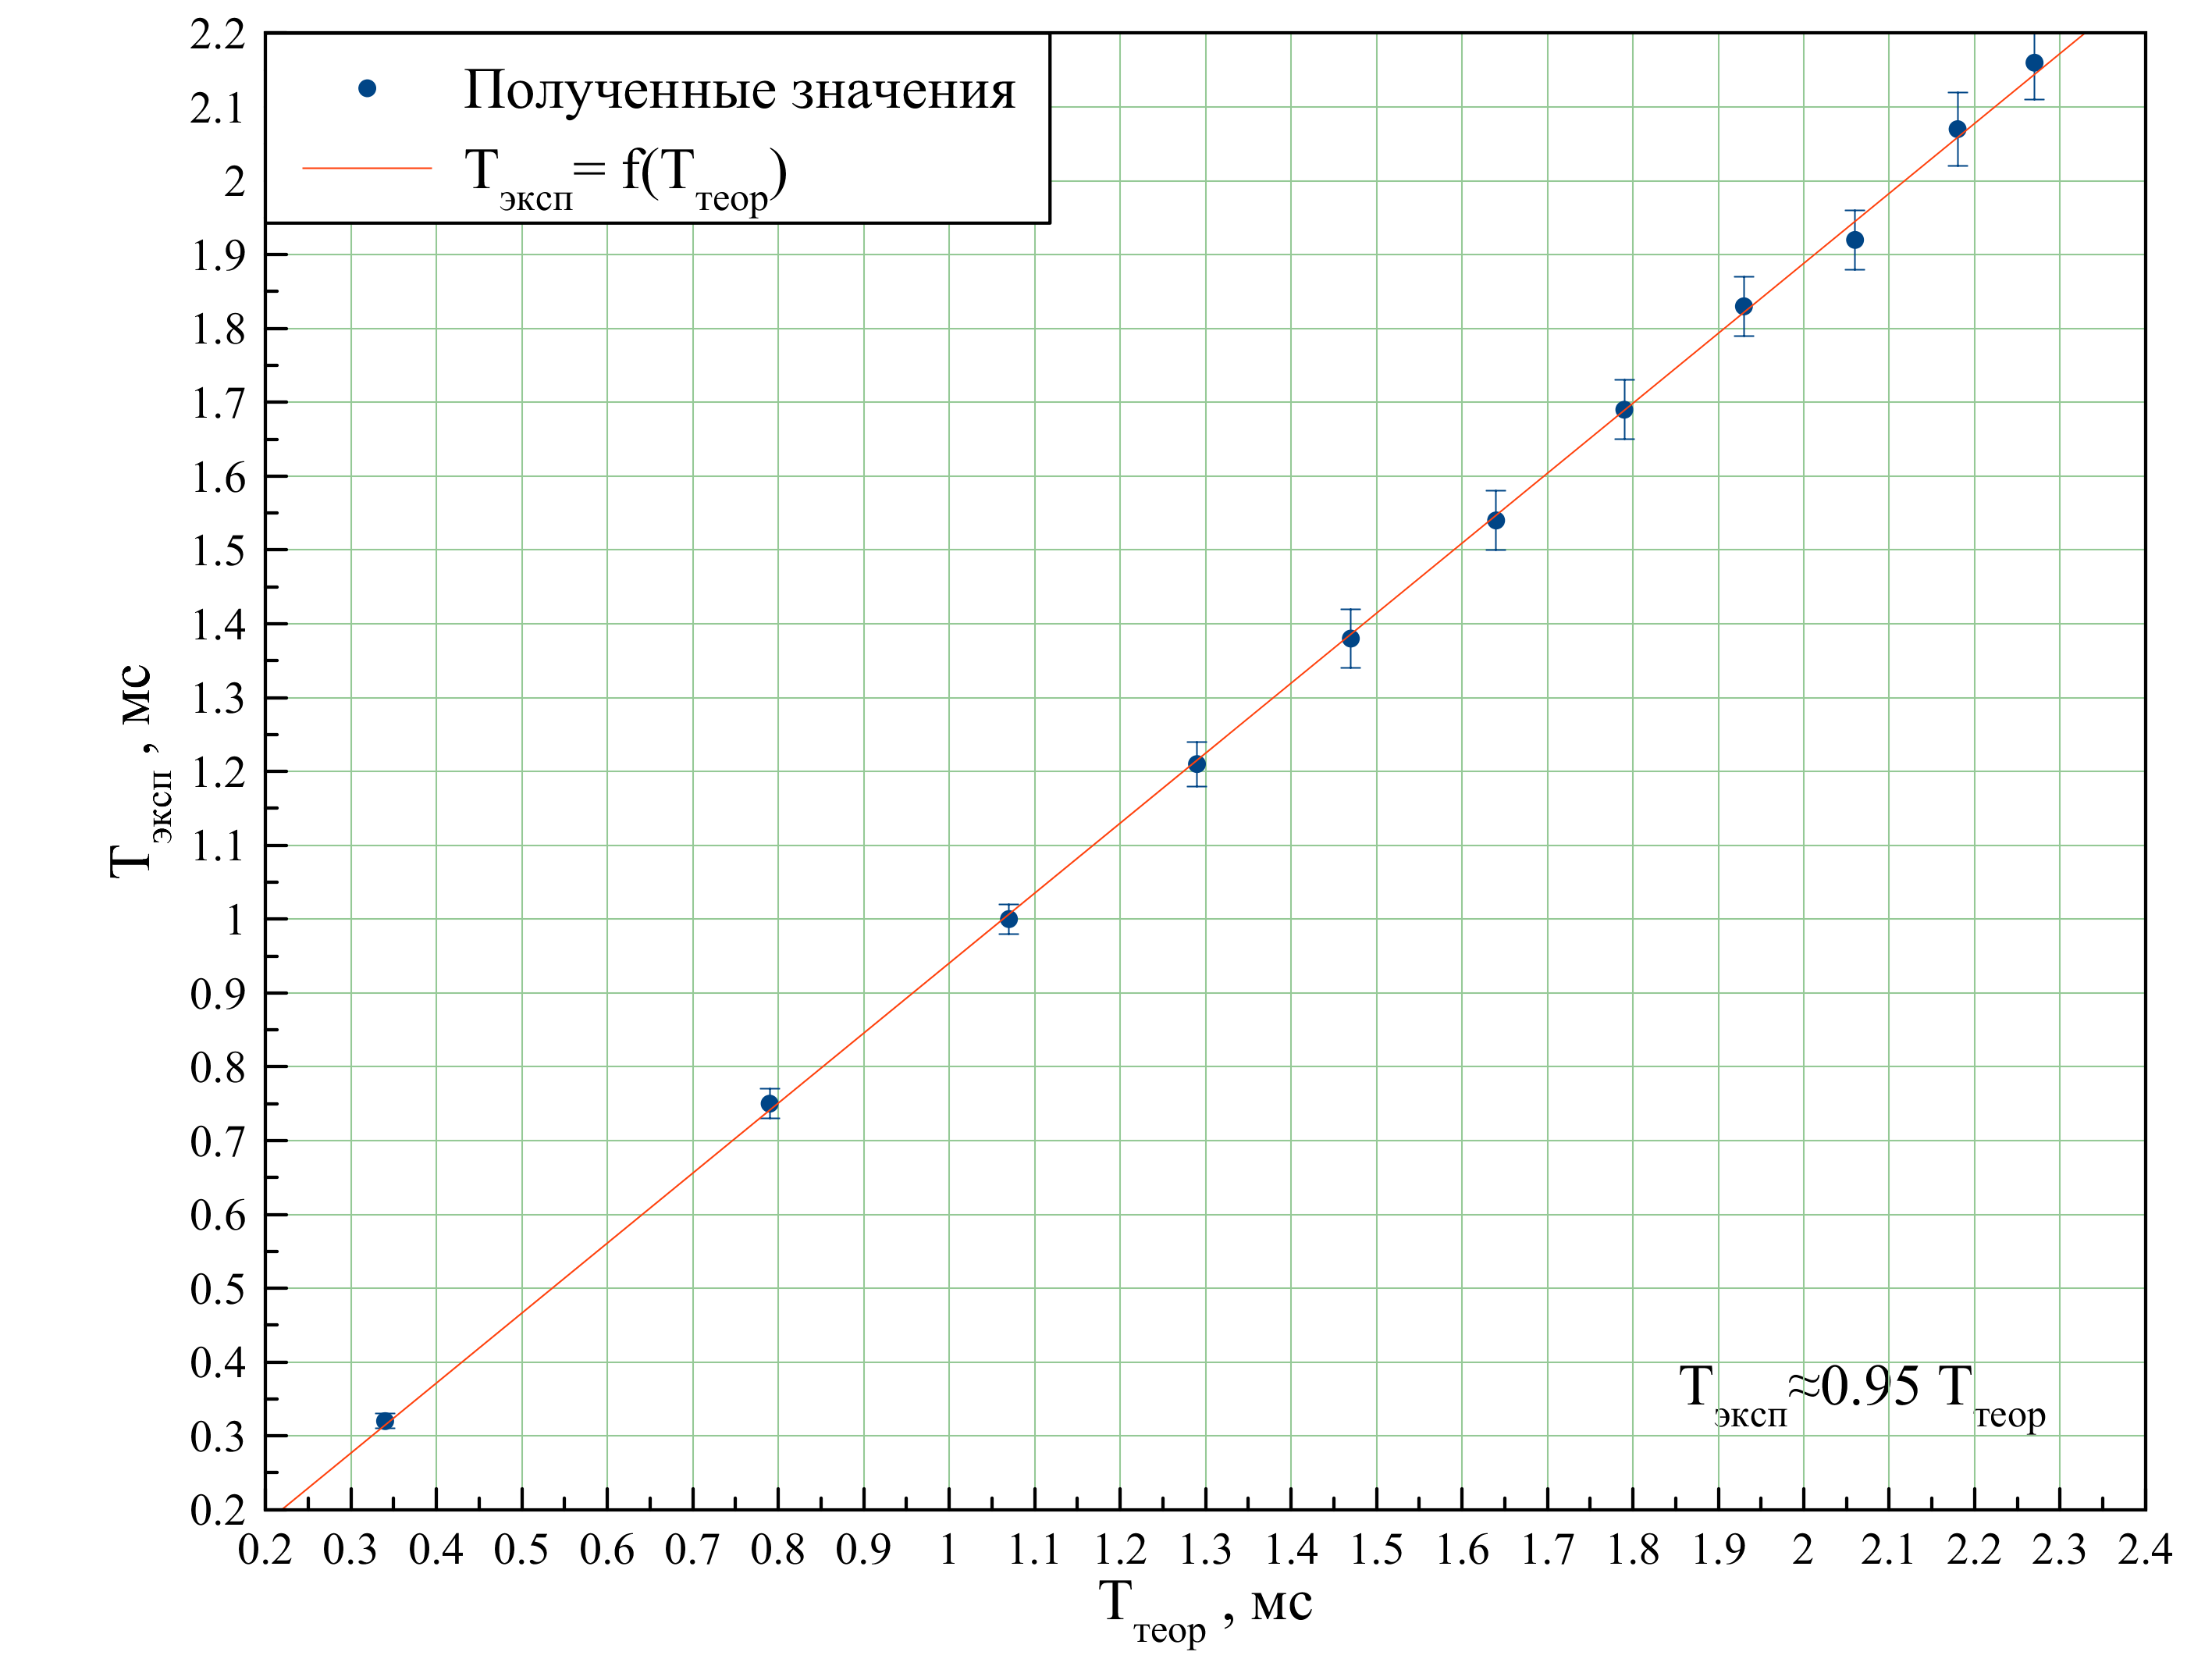
\includegraphics[width = 0.8\textwidth]{graph1}
	\caption{График функции $T_{\text{эксп}} = f(T_{\text{теор}})$.}
	\label{graph1}
\end{figure}

Найдём тангенс угла наклона с помощью метода наименьших квадратов $$k = \dfrac{<T_{\text{теор}} T_{\text{эксп}}>}{<T_{\text{теор}}^2>},  ~ \sigma_k = \dfrac{1}{11}\sqrt{\dfrac{<T_{\text{эксп}}^2>}{<T_{\text{теор}}^2>} - k^2}$$,

тогда
\begin{equation*}
\fbox{$T_{\text{эксп}} = (0,940\pm 0,001)T_{\text{теор}}$}
\end{equation*}

\subsection{Исследование логарифмического декремента затухания.}
Рассчитаем значение $R_{\text{конт}}$(сопротивление контура
 состоит из сопротивления магазина $R$ и омического сопротивления катушки $R_{L}$). Построим график в координатах\\ 
 $1/\Theta^{2} = f[1/(R^{2}_{\text{конт}})]$. Примем обозначения $1/\Theta^{2} = Y$, $1/(R^{2}_{\text{конт}}) = X$. Необходимые измерения возьмём из таблицы \ref{table2}
 
 \begin{table}[H]
 	\centering
 	\caption{Данные для построения графика $1/\Theta^{2} = f[1/(R^{2}_{\text{конт}})]$. }
 	\label{tabel6}
 	\begin{tabular}{|c|c|c|}
 		\hline
 		$R_{\text{конт}},$ Ом & $1/(R^{2}_{\text{конт}}), 1/\text{Ом$^2$}\times10^{-7}$  & $1/\Theta^2$\\ \hline
 		1010  & 9,80                                          & 1,99                      \\ \hline
 		1260  & 6,29                                          & 1,26                      \\ \hline
 		1510  & 4,39                                          & 0,87                      \\ \hline
 		1760  & 3,23                                          & 0,72                      \\ \hline
 		2010  & 2,48                                          & 0,52                      \\ \hline
 		2260  & 1,96                                          & 0,47                      \\ \hline
 		2510  & 1,59                                          & 0,34                      \\ \hline
 		2760  & 1,31                                          & 0,29                      \\ \hline
 		3010  & 1,10                                          & 0,21                      \\ \hline
 	\end{tabular}
 \end{table}

\begin{figure}[H]
	\centering
	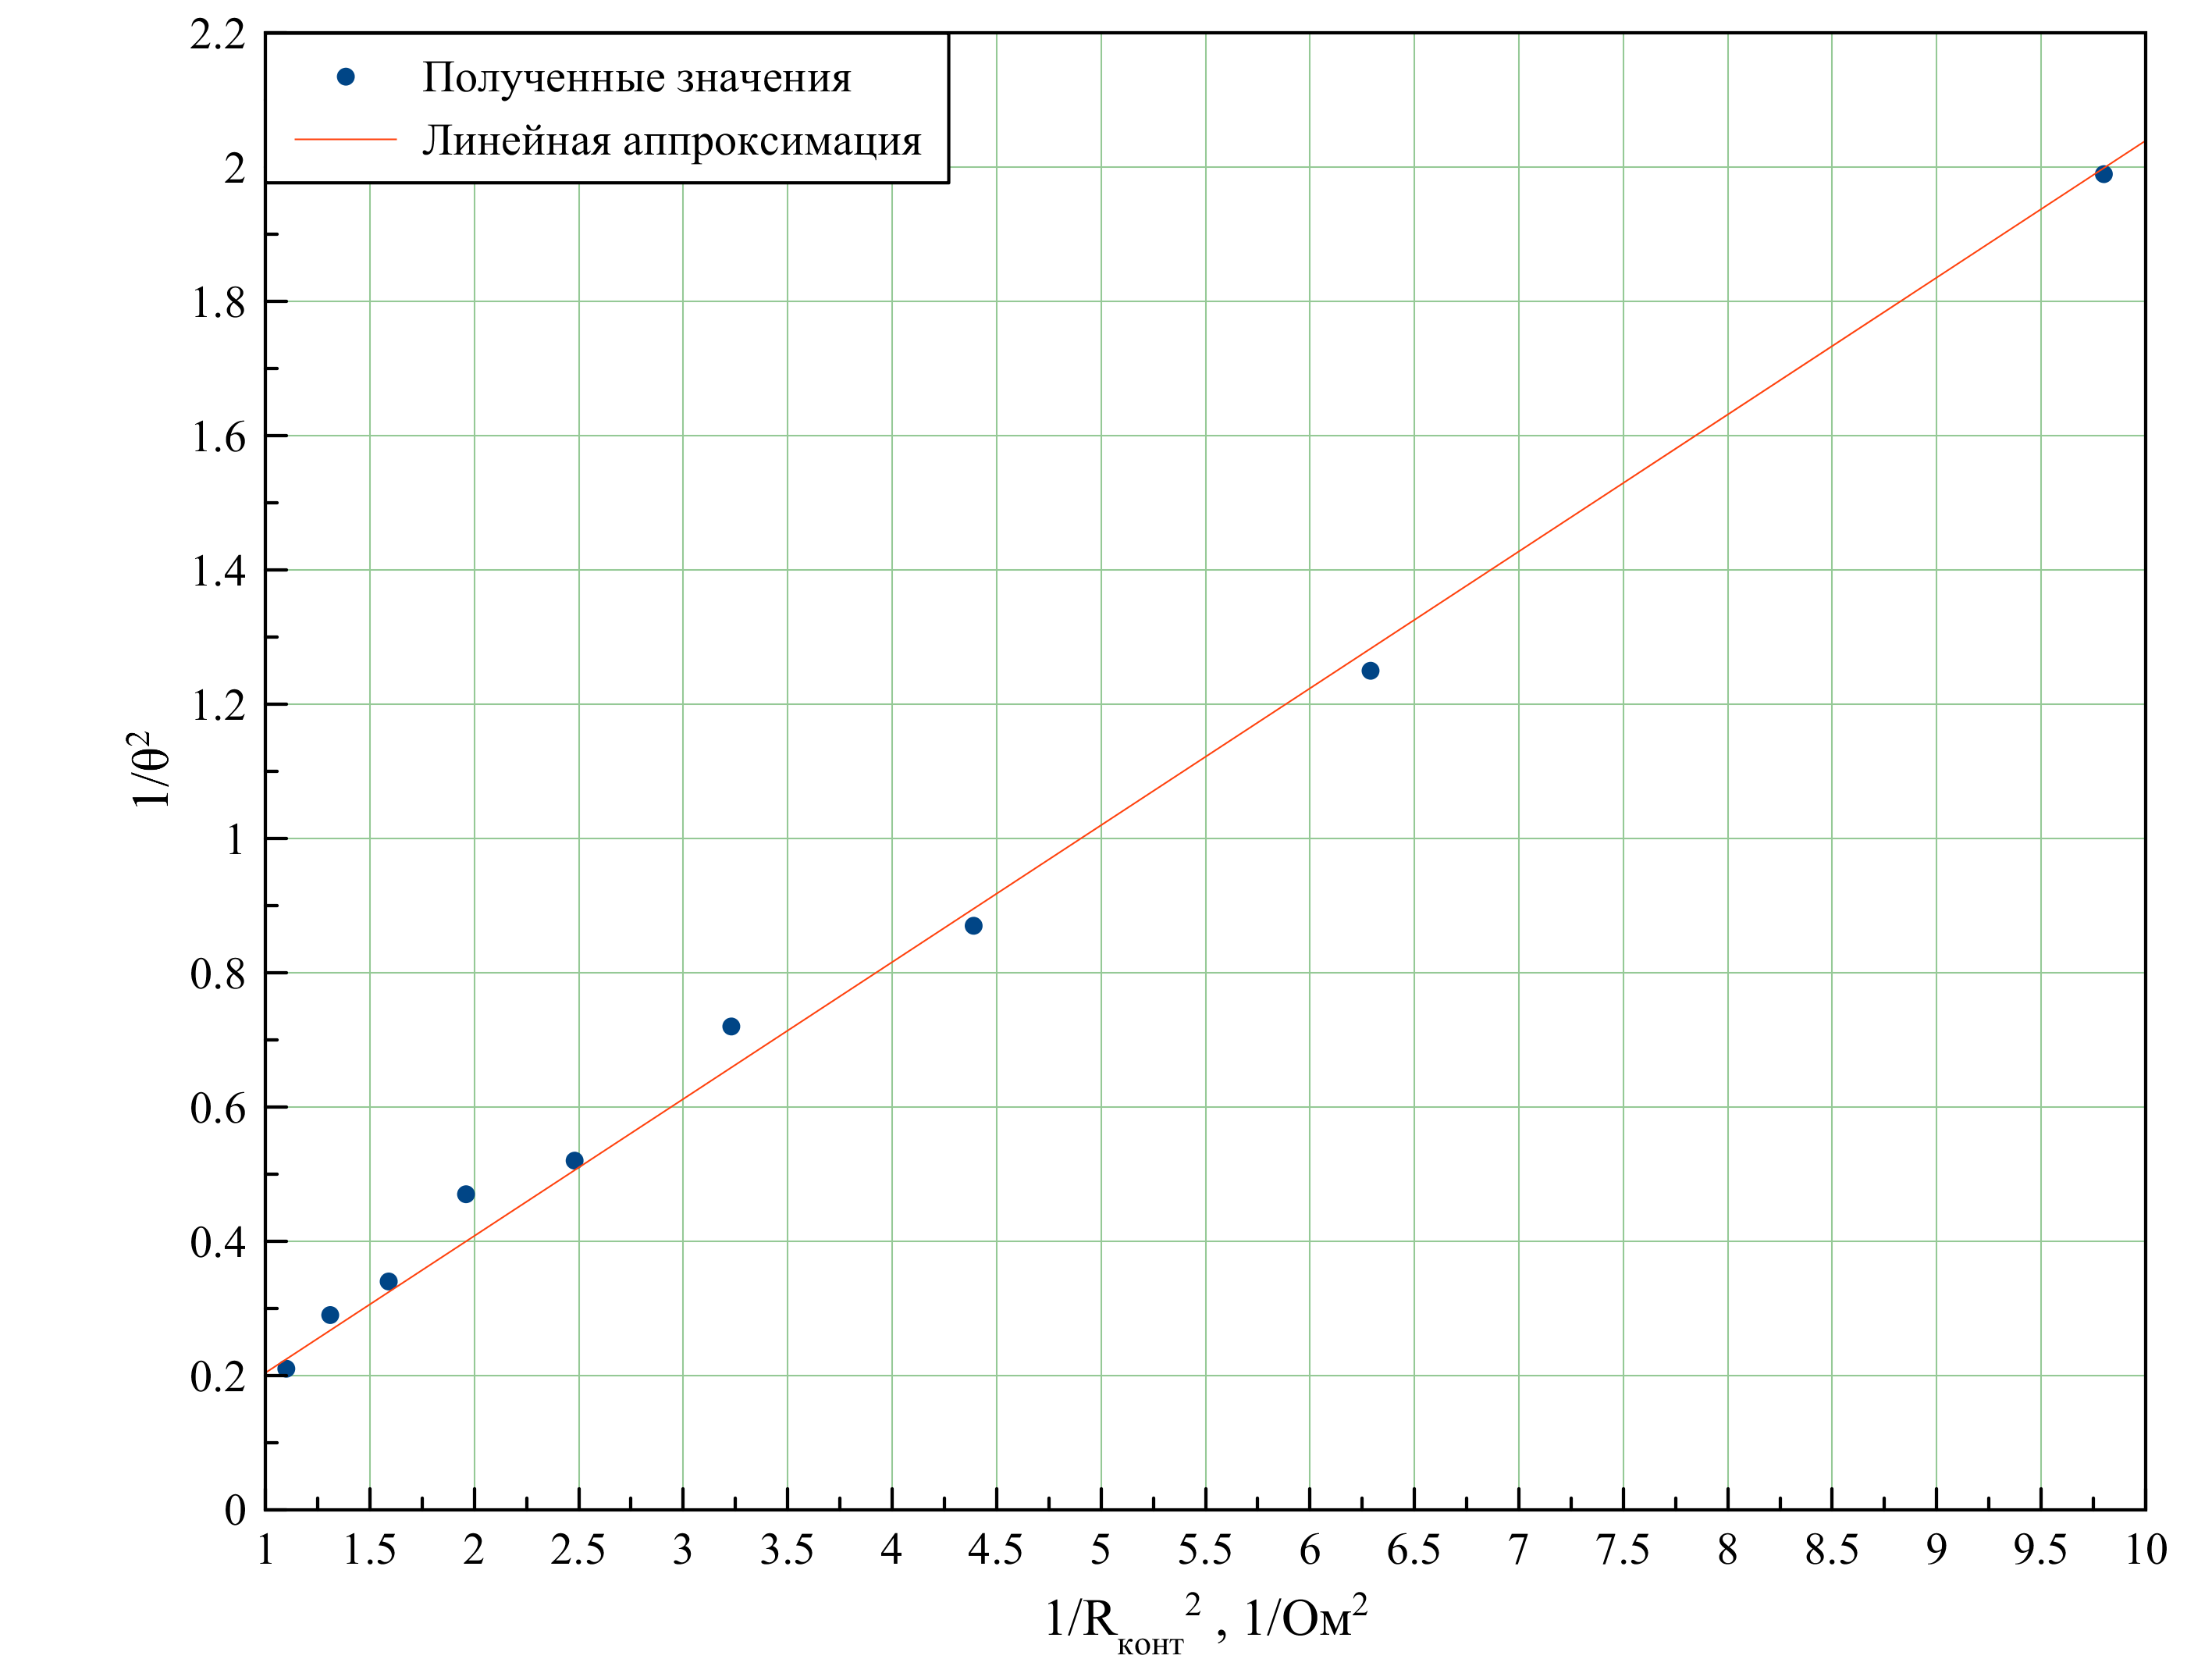
\includegraphics[width = 0.8\textwidth]{graph2}
	\caption{График функции $1/\Theta^{2} = f[1/(R^{2}_{\text{конт}})]$.}
	\label{graph2}
\end{figure}
Найдём тангенс угла наклона $k$ прямой графика, изображённого на рис. \ref{graph2}, с помощью метода наименьших квадратов по формуле $$ k = \dfrac{\langle XY\rangle}{\langle X^2\rangle},~ \sigma_{k} = \dfrac{1}{\sqrt{n}}\sqrt{\dfrac{\langle Y^2 \rangle}{\langle X^2 \rangle} - k^2}$$.

Тогда имеем $$k = (2044038\pm 26622) \text{Ом$^2$}$$.

Из формулы $R_{\text{кр}} = 2\pi \sqrt{\Delta Y/\Delta X}$ получаем
\begin{equation}
\fbox{\text{$
R_{\text{кр}} = (8973 \pm 58)\text{Ом}$}}
\end{equation}

Рассчитаем теоретическое значение $R_{\text{кр}} = 2\sqrt{L/C}$, где $L \approx 145 \text{мГн}$ и $ C \approx 0,007 \text{мкФ}$.
\begin{equation}
\fbox{\text{$
		R_{\text{кр}} \approx 9102\text{Ом}$}}
\end{equation}

Рассчитаем добротность контура Q для максимального и минимального значений $\Theta$ по картине затухающих колебаний и по спирали. Для этого воспользуемся формулой $Q=\pi/\Theta$. Сравним полученные значения с теоретическими, рассчитанными по формуле $Q=1/R\sqrt{L/C}$. Найдем погрешности измерения $R_{\text{кр}}$ и $Q$ по отношению к табличному значению. Сведём результаты эксперимента в таблицу \ref{table7}

\begin{table}[H]
	\centering
	\caption{Итоговые результаты эксперимента.}
	\label{table7}
	\begin{tabular}{|c|c|c|c|c|c|c|c|}
		\hline
		\multirow{2}{*}{Lкат, мГн} & \multicolumn{3}{c|}{Rкр, Ом}                                            & R, кОм & \multicolumn{3}{c|}{Q}                                                                                                                                                     \\ \cline{2-8} 
		& Теор.                 & Подбор                & Граф.                   &        & Теор. & $f(\Theta)$                                                                    & Спираль                                                                           \\ \hline
		\multirow{2}{*}{145}       & \multirow{2}{*}{9102} & $10000 \pm 898$       & $8973 \pm 129$          & 3      & 1,52  & \begin{tabular}[c]{@{}c@{}}$1,45\pm 0,07$\\ ($\varepsilon = 5\%$)\end{tabular} & \begin{tabular}[c]{@{}c@{}}$1,54 \pm 0,02$\\ ($\varepsilon = 1,3\%$)\end{tabular} \\ \cline{5-8} 
		&                       & ($\varepsilon = 9\%$) & ($\varepsilon = 1,5\%$) & 1      & 4,55  & \begin{tabular}[c]{@{}c@{}}$4,42\pm 0,13$\\ ($\varepsilon = 3\%$)\end{tabular} & \begin{tabular}[c]{@{}c@{}}$4,69\pm 0,14$\\ ($\varepsilon = 3\%$)\end{tabular}    \\ \hline
	\end{tabular}
\end{table}

\section{Вывод.}

Рассчитанные значения $R_{\text{кр}}$ и $\Theta$ практически совпадают с теоретическими (относительные погрешности не превышают $5\%$).

При определении $R_{\text{кр}}$, несомненно, предпочтительнее графический метод перед методом подбора, так как определить на глаз момент перехода критического режима в апериодический довольно сложно.

В ходе работы были измерены с довольно высокой точностью:

а)период свободных колебаний контура

б)критическое сопротивление

в)декремент затухания

г)добротность контура.



\end{document}